\documentclass[12pt]{article}
\usepackage[utf8]{inputenc}
\usepackage[english]{babel}
\usepackage[margin=1in]{geometry}
\usepackage{setspace}
\usepackage{amsmath}
\usepackage{graphicx}
\usepackage[authoryear,round]{natbib}
\usepackage{hyperref}
\usepackage{booktabs}
\usepackage{longtable}
\usepackage{array}
\usepackage{multirow}
\usepackage{tikz}
\usetikzlibrary{shapes.geometric, arrows, positioning, fit, backgrounds}

\doublespacing
\title{\textbf{Research Design and Methodology:\\Complete Specification}}
\date{}

\begin{document}
\maketitle

\section{Study Design Overview}

This study employed a 2 (Agent Memory Function: +MAPK vs. $-$MAPK) $\times$ 2 (Agent Personality: Introvert vs. Extrovert) between-subjects factorial design to investigate how agent memory capabilities and personality characteristics influence human trust calibration in human-AI collaboration. The study was conducted \textbf{entirely online} using a remote VR paradigm, allowing participants to complete the experiment in their own homes using their personal Oculus Quest 2 headsets.

\subsection{Research Questions}

\begin{enumerate}
    \item \textbf{RQ1}: Does agent memory function (+MAPK vs. $-$MAPK) affect trust calibration in human-AI teams?
    \item \textbf{RQ2}: Does agent personality (Introvert vs. Extrovert) influence trust formation and maintenance?
    \item \textbf{RQ3}: Does personality matching (congruence between human and agent personality) moderate trust dynamics?
    \item \textbf{RQ4}: How do these factors interact to shape behavioral trust compliance patterns?
\end{enumerate}

\subsection{Experimental Conditions}

Participants were randomly assigned to one of four experimental conditions:

\begin{figure}[h]
\centering
\includegraphics[width=0.7\textwidth]{../03_FIGURES_MAIN/Fig_Experimental_Design.png}
\caption{2 × 2 Factorial Experimental Design showing the four conditions combining agent memory function (±MAPK) and agent personality (Introvert vs. Extrovert). Each condition contained 23 participants (N = 92 total). The design allows examination of main effects of memory function and agent personality, as well as their interaction effects on trust calibration.}
\label{fig:experimental_design}
\end{figure}

\begin{table}[h]
\centering
\caption{2 $\times$ 2 Factorial Design Conditions}
\begin{tabular}{lcc}
\toprule
& \textbf{Introvert Agent} & \textbf{Extrovert Agent} \\
\midrule
\textbf{+MAPK (With Memory)} & Condition 1 (\textit{n} = 23) & Condition 2 (\textit{n} = 23) \\
\textbf{$-$MAPK (Without Memory)} & Condition 3 (\textit{n} = 23) & Condition 4 (\textit{n} = 23) \\
\bottomrule
\end{tabular}
\end{table}

\textbf{Target sample size}: \textit{N} = 92 (23 participants per cell)

\textbf{Power analysis}: Based on pilot testing (\textit{n} = 12), medium effect sizes ($f$ = 0.25, $d$ = 0.50) for memory and personality effects were anticipated. With \textit{n} = 23 per cell, power = 0.80 for detecting medium effects at $\alpha$ = .05.

\section{Participant Recruitment}

\subsection{Recruitment Platform: Prolific}

Participants were recruited through \textbf{Prolific} (https://www.prolific.co), an online research participant platform. Unlike typical online studies, this study required participants to have specialized equipment and VR expertise.

\subsection{Eligibility Criteria}

Prolific's pre-screening system filtered participants based on strict VR-related requirements:

\begin{table}[h]
\centering
\caption{Participant Eligibility Criteria}
\begin{tabular}{p{0.35\textwidth}p{0.55\textwidth}}
\toprule
\textbf{Criterion} & \textbf{Requirement} \\
\midrule
\textbf{VR Equipment Ownership} & Must own an \textbf{Oculus Quest 2} headset \\
\midrule
\textbf{VR Experience Level} & Must play VR games/applications \textbf{at least 3 times per week} \\
\midrule
\textbf{VR Familiarity} & Self-reported VR proficiency $\geq$ 7/10 \\
\midrule
\textbf{Technical Capability} & Able to install APK files on Quest 2 (sideloading experience preferred) \\
\midrule
Age & 18 years or older \\
\midrule
Fluency & English fluency (self-reported 8/10 or higher) \\
\midrule
Vision & Normal or corrected-to-normal vision (compatible with VR headset use) \\
\midrule
Geographic location & United States or United Kingdom \\
\midrule
Approval rate & $\geq$ 95\% approval rate on previous Prolific studies \\
\midrule
Device access & Access to computer for online pre/post surveys \\
\midrule
Availability & Available to complete study within 7 days of acceptance \\
\bottomrule
\end{tabular}
\end{table}

\textbf{Rationale for VR expertise requirement}:
\begin{itemize}
    \item Minimized learning effects and VR sickness
    \item Enabled focus on trust dynamics rather than VR adaptation
    \item Ensured participants could complete task independently without technical support
    \item Reduced attrition due to VR discomfort or technical difficulties
\end{itemize}

\subsection{Compensation Structure}

\subsubsection{Base Compensation}

All participants received \textbf{\$25 USD} base compensation for:
\begin{itemize}
    \item Pre-study online survey (10--15 minutes)
    \item Downloading and installing VR application (5--10 minutes)
    \item Completing VR navigation task (30--45 minutes)
    \item Post-task online surveys (20--30 minutes)
\end{itemize}

\textbf{Total time commitment}: 1.5--2 hours

\textbf{Hourly rate}: \$25 for 1.5--2 hours = \$12.50--\$16.67/hour (exceeds Prolific minimum wage standards of \$12/hour USD)

\subsubsection{Performance Bonus Incentive}

To encourage genuine task engagement and efficient decision-making, a \textbf{performance bonus} was offered:

\textbf{Top 1\% performer}: Additional \textbf{\$5 bonus} (\$30 total compensation)

\textbf{Performance criteria}:
\begin{itemize}
    \item Task completion time (faster completion preferred)
    \item Decision accuracy (choosing correct paths)
    \item Minimal backtracking (fewer errors)
\end{itemize}

\textbf{Performance calculation}:
\begin{equation}
\text{Performance Score} = 0.50 \times \text{Accuracy} + 0.30 \times (1 - \text{Normalized Time}) + 0.20 \times (1 - \text{Normalized Backtracks})
\end{equation}

\textbf{Top 1\% threshold}: The single participant (\textit{n} = 1 out of 92) with the highest performance score received the \$5 bonus.

\textbf{Transparency}: Participants were informed of the bonus structure in the informed consent but were not shown real-time performance scores during the task to prevent interference with natural trust calibration.

\subsection{Sample Demographics}

Final sample (\textit{N} = 92) demographics:

\begin{table}[h]
\centering
\caption{Sample Demographics}
\begin{tabular}{lrr}
\toprule
\textbf{Characteristic} & \textbf{Count / M (SD)} & \textbf{Percentage / Range} \\
\midrule
\textbf{Age} & 28.4 (7.2) & 18--54 \\
\midrule
\textbf{Gender} & & \\
\quad Female & 47 & 51.1\% \\
\quad Male & 43 & 46.7\% \\
\quad Non-binary & 2 & 2.2\% \\
\midrule
\textbf{Education} & & \\
\quad High school & 8 & 8.7\% \\
\quad Some college & 15 & 16.3\% \\
\quad Bachelor's degree & 52 & 56.5\% \\
\quad Graduate degree & 17 & 18.5\% \\
\midrule
\textbf{VR Experience (Years)} & 2.8 (1.4) & 0.5--7 \\
\midrule
\textbf{VR Usage Frequency} & & \\
\quad 3 times/week & 38 & 41.3\% \\
\quad 4--5 times/week & 32 & 34.8\% \\
\quad Daily & 22 & 23.9\% \\
\midrule
\textbf{Personality (BFI Extraversion)} & 3.24 (0.68) & 1.50--4.88 \\
\quad Introverts (BFI $<$ 3.0) & 38 & 41.3\% \\
\quad Extroverts (BFI $\geq$ 3.0) & 54 & 58.7\% \\
\bottomrule
\end{tabular}
\end{table}

\section{Random Assignment Procedure}

\subsection{Randomization Strategy}

\textbf{Randomization method}: Block randomization with equal distribution

\textbf{Randomization software}: Qualtrics randomizer

\subsubsection{Block Randomization Implementation}

\textbf{Block size}: 4 participants per block

\textbf{Procedure}:
\begin{enumerate}
    \item Participants completed informed consent and pre-screening
    \item Upon meeting all eligibility criteria, Qualtrics randomizer assigned participant to 1 of 4 conditions
    \item Assignment was balanced using block randomization (every 4 participants included exactly 1 per condition)
    \item Condition assignment determined which APK version participant received
    \item 23 complete blocks ($23 \times 4 = 92$ total participants)
\end{enumerate}

\textbf{Participant blinding}: Participants were \textbf{not informed} of:
\begin{itemize}
    \item The existence of multiple experimental conditions
    \item Which condition they were assigned to
    \item The specific experimental manipulations (memory function, personality type)
\end{itemize}

\textbf{Participants were told}: ``You will work with an AI agent to navigate a virtual maze. The agent will provide guidance to help you find the correct path.''

\section{Study Procedure}

\subsection{Overview of Remote VR Paradigm}

This study employed a \textbf{fully remote data collection paradigm}:
\begin{itemize}
    \item Participants completed the study \textbf{at home} using their personal Oculus Quest 2 headsets
    \item VR application delivered as \textbf{APK file} (Android application package)
    \item No in-person lab visits required
    \item Self-paced completion within 7-day window
\end{itemize}

\textbf{Advantages of remote VR approach}:
\begin{enumerate}
    \item \textbf{Ecological validity}: Participants interacted with VR in natural home environment
    \item \textbf{Geographic diversity}: No geographic constraints (US/UK recruitment)
    \item \textbf{Participant comfort}: Familiar equipment and environment reduced anxiety
    \item \textbf{Scalability}: Enabled larger sample collection without lab space constraints
    \item \textbf{Cost-effectiveness}: No equipment procurement or lab space rental needed
\end{enumerate}

\subsection{Complete Study Flow}

\begin{figure}[p]
\centering
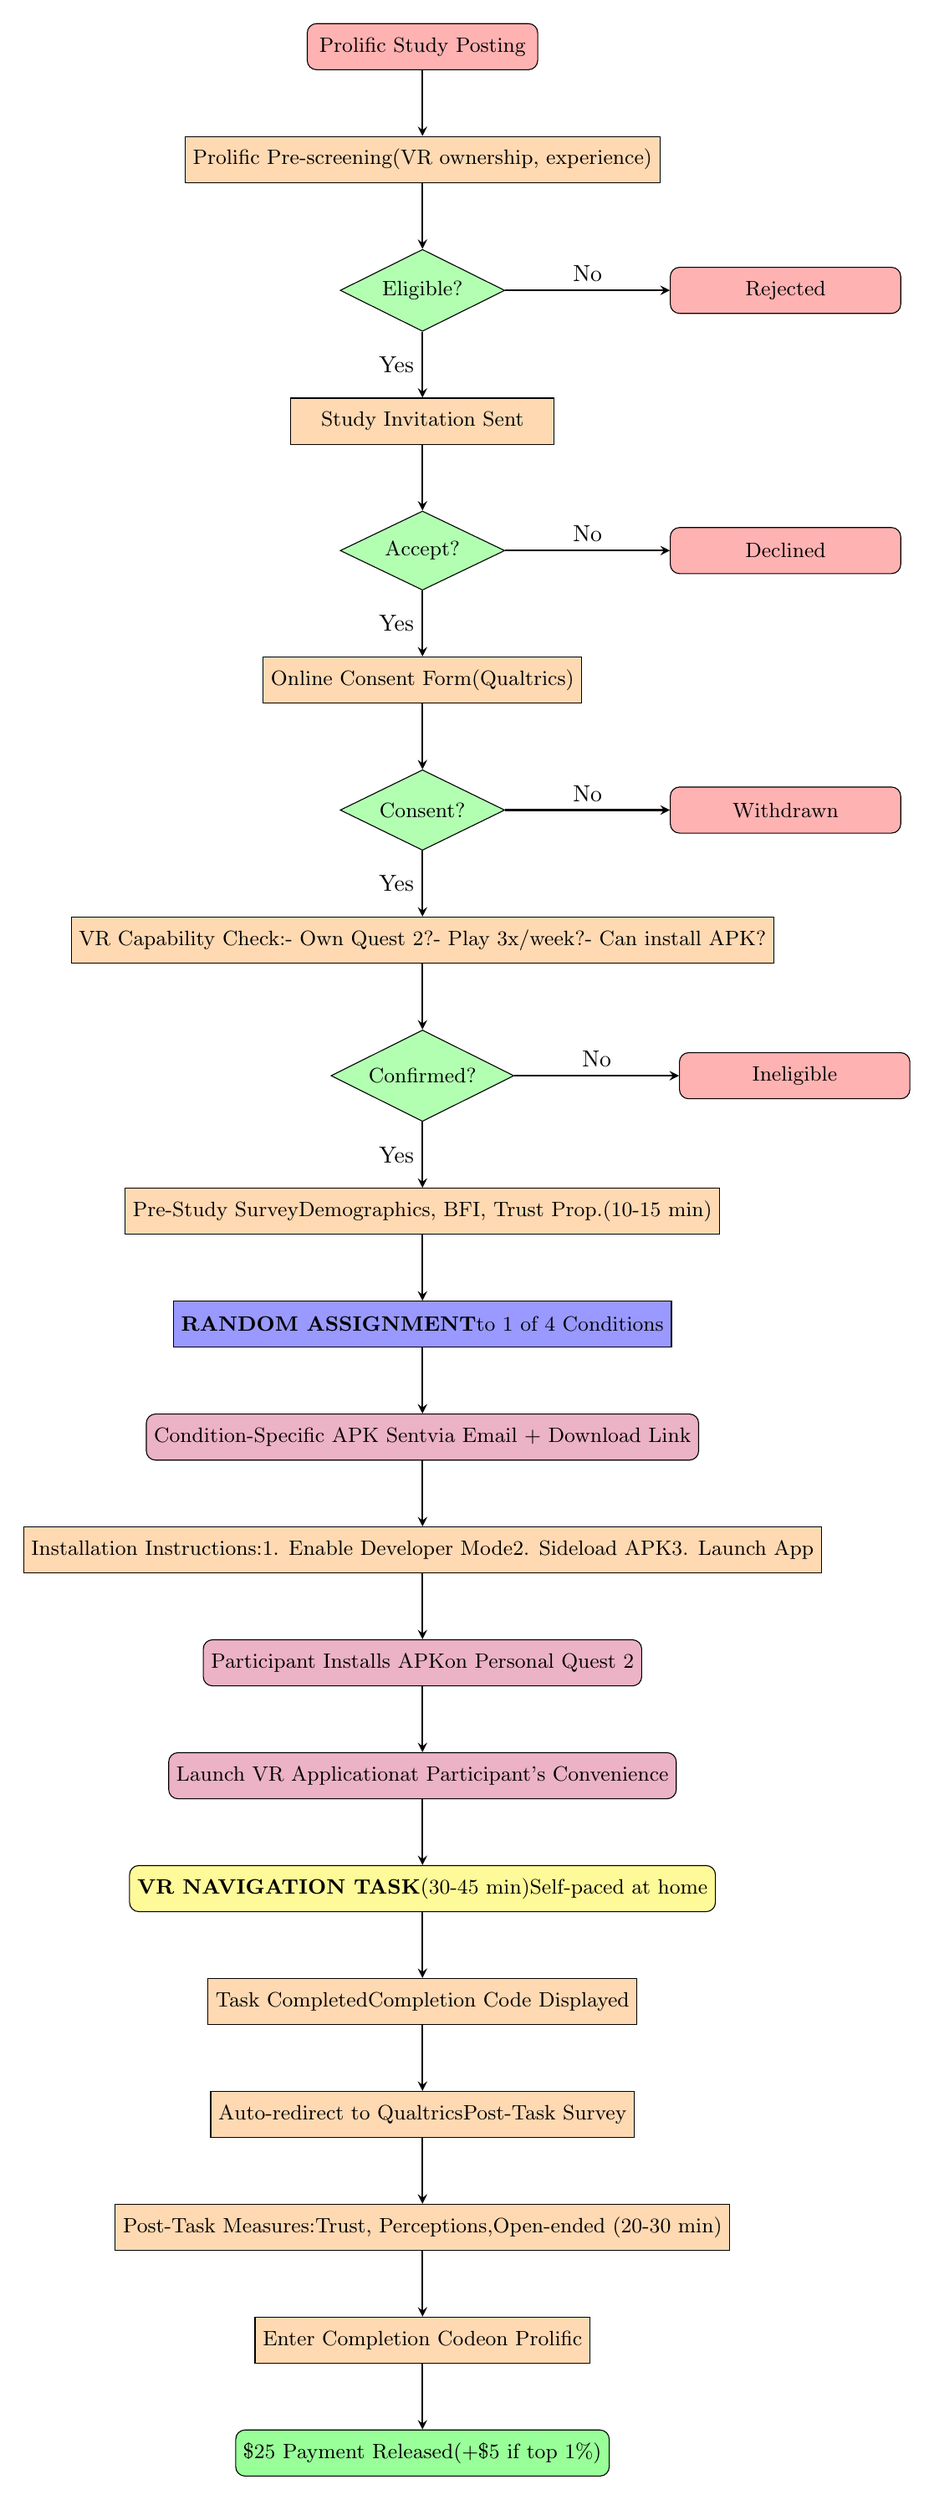
\begin{tikzpicture}[
    node distance=1cm,
    startstop/.style={rectangle, rounded corners, minimum width=3.5cm, minimum height=0.7cm, text centered, draw=black, fill=red!30, font=\small},
    process/.style={rectangle, minimum width=4cm, minimum height=0.7cm, text centered, draw=black, fill=orange!30, font=\small},
    decision/.style={diamond, aspect=2, minimum width=2.5cm, minimum height=0.7cm, text centered, draw=black, fill=green!30, font=\small},
    vr/.style={rectangle, rounded corners, minimum width=4cm, minimum height=0.7cm, text centered, draw=black, fill=purple!30, font=\small},
    arrow/.style={thick,->,>=stealth}
]

% Start
\node (start) [startstop] {Prolific Study Posting};
\node (prescreen) [process, below=of start] {Prolific Pre-screening\\(VR ownership, experience)};
\node (eligible) [decision, below=of prescreen] {Eligible?};
\node (reject) [startstop, right=2.5cm of eligible] {Rejected};

% Consent
\node (invite) [process, below=of eligible] {Study Invitation Sent};
\node (accept) [decision, below=of invite] {Accept?};
\node (decline) [startstop, right=2.5cm of accept] {Declined};
\node (consent) [process, below=of accept] {Online Consent Form\\(Qualtrics)};
\node (consentdec) [decision, below=of consent] {Consent?};
\node (withdraw1) [startstop, right=2.5cm of consentdec] {Withdrawn};

% Pre-screening questions
\node (vrchecks) [process, below=of consentdec] {VR Capability Check:\\- Own Quest 2?\\- Play 3x/week?\\- Can install APK?};
\node (vrconfirm) [decision, below=of vrchecks] {Confirmed?};
\node (reject2) [startstop, right=2.5cm of vrconfirm] {Ineligible};

% Pre-survey and randomization
\node (presurvey) [process, below=of vrconfirm] {Pre-Study Survey\\Demographics, BFI, Trust Prop.\\(10-15 min)};
\node (randomize) [process, below=of presurvey, fill=blue!40] {\textbf{RANDOM ASSIGNMENT}\\to 1 of 4 Conditions};

% APK delivery
\node (apkdelivery) [vr, below=of randomize] {Condition-Specific APK Sent\\via Email + Download Link};
\node (instructions) [process, below=of apkdelivery] {Installation Instructions:\\1. Enable Developer Mode\\2. Sideload APK\\3. Launch App};

% VR task
\node (install) [vr, below=of instructions] {Participant Installs APK\\on Personal Quest 2};
\node (launch) [vr, below=of install] {Launch VR Application\\at Participant's Convenience};
\node (vrtask) [vr, below=of launch, fill=yellow!40] {\textbf{VR NAVIGATION TASK}\\(30-45 min)\\Self-paced at home};

% Post-task
\node (complete) [process, below=of vrtask] {Task Completed\\Completion Code Displayed};
\node (redirect) [process, below=of complete] {Auto-redirect to Qualtrics\\Post-Task Survey};
\node (postsurvey) [process, below=of redirect] {Post-Task Measures:\\Trust, Perceptions,\\Open-ended (20-30 min)};
\node (code) [process, below=of postsurvey] {Enter Completion Code\\on Prolific};
\node (payment) [startstop, below=of code, fill=green!40] {\$25 Payment Released\\(+\$5 if top 1\%)};

% Arrows
\draw [arrow] (start) -- (prescreen);
\draw [arrow] (prescreen) -- (eligible);
\draw [arrow] (eligible) -- node[anchor=south] {No} (reject);
\draw [arrow] (eligible) -- node[anchor=east] {Yes} (invite);
\draw [arrow] (invite) -- (accept);
\draw [arrow] (accept) -- node[anchor=south] {No} (decline);
\draw [arrow] (accept) -- node[anchor=east] {Yes} (consent);
\draw [arrow] (consent) -- (consentdec);
\draw [arrow] (consentdec) -- node[anchor=south] {No} (withdraw1);
\draw [arrow] (consentdec) -- node[anchor=east] {Yes} (vrchecks);
\draw [arrow] (vrchecks) -- (vrconfirm);
\draw [arrow] (vrconfirm) -- node[anchor=south] {No} (reject2);
\draw [arrow] (vrconfirm) -- node[anchor=east] {Yes} (presurvey);
\draw [arrow] (presurvey) -- (randomize);
\draw [arrow] (randomize) -- (apkdelivery);
\draw [arrow] (apkdelivery) -- (instructions);
\draw [arrow] (instructions) -- (install);
\draw [arrow] (install) -- (launch);
\draw [arrow] (launch) -- (vrtask);
\draw [arrow] (vrtask) -- (complete);
\draw [arrow] (complete) -- (redirect);
\draw [arrow] (redirect) -- (postsurvey);
\draw [arrow] (postsurvey) -- (code);
\draw [arrow] (code) -- (payment);

\end{tikzpicture}
\caption{Complete Remote VR Study Flow}
\end{figure}

\clearpage

\subsection{Detailed Procedure Timeline}

\subsubsection{Phase 1: Online Recruitment and Consent (Days 1--2)}

\textbf{Step 1: Prolific Study Posting}
\begin{itemize}
    \item Study posted on Prolific with detailed description
    \item Title: ``VR Navigation Study with AI Agent (Requires Oculus Quest 2)''
    \item Estimated time: 1.5--2 hours
    \item Payment: \$25 (+ \$5 performance bonus for top 1\%)
    \item Special requirements clearly stated: Quest 2 ownership, 3x/week VR usage
\end{itemize}

\textbf{Step 2: Pre-screening}
\begin{itemize}
    \item Prolific's automated system filters for:
    \begin{itemize}
        \item VR headset ownership (Quest 2 specifically)
        \item VR usage frequency ($\geq$ 3 times/week)
        \item Age ($\geq$ 18)
        \item Location (US/UK)
        \item Approval rate ($\geq$ 95\%)
    \end{itemize}
\end{itemize}

\textbf{Step 3: Study Acceptance and Consent}
\begin{itemize}
    \item Eligible participants click ``Accept Study''
    \item Redirected to Qualtrics consent form
    \item Consent form includes:
    \begin{itemize}
        \item Study purpose (investigating trust in AI navigation agents)
        \item Procedures (VR navigation task at home, online surveys)
        \item Time commitment (1.5--2 hours)
        \item Compensation (\$25 base + possible \$5 bonus)
        \item Risks (mild VR discomfort, though unlikely given experience level)
        \item Data confidentiality and privacy protections
        \item Right to withdraw at any time
        \item Contact information for questions
    \end{itemize}
    \item Participant provides electronic signature to continue
\end{itemize}

\textbf{Step 4: VR Capability Confirmation}
\begin{itemize}
    \item After consent, participants answer confirmation questions:
    \begin{enumerate}
        \item ``Do you currently own an Oculus Quest 2 headset?'' (Yes/No)
        \item ``How many times per week do you typically use VR?'' (Dropdown: 3, 4, 5, 6, 7+)
        \item ``Have you ever installed APK files on your Quest 2 (sideloading)?'' (Yes/No/Willing to learn)
        \item ``Rate your comfort level with VR technology'' (1--10 scale)
    \end{enumerate}
    \item Participants who answer ``No'' to Quest 2 ownership or ``Less than 3'' to weekly usage are excluded
\end{itemize}

\textbf{Step 5: Pre-Study Survey (10--15 minutes)}
\begin{itemize}
    \item Demographics: Age, gender, education, VR experience history
    \item Big Five Inventory (BFI-10): Measures personality dimensions, especially extraversion
    \item Propensity to Trust Technology Scale: Baseline technology trust tendencies
    \item VR experience details: Types of VR applications used, comfort level
\end{itemize}

\textbf{Step 6: Random Assignment}
\begin{itemize}
    \item Upon completing pre-survey, Qualtrics randomizer assigns participant to 1 of 4 conditions
    \item Assignment determines which APK file participant receives
    \item Participant shown: ``Thank you! You will receive your study materials within 24 hours.''
\end{itemize}

\subsubsection{Phase 2: APK Distribution and Installation (Days 2--3)}

\textbf{Step 7: APK Delivery}
\begin{itemize}
    \item Within 24 hours, participant receives email containing:
    \begin{itemize}
        \item Personalized greeting with Participant ID
        \item Direct download link to condition-specific APK file
        \item Backup Google Drive link (in case primary link fails)
        \item APK file name: \texttt{NavigationTask\_[ParticipantID].apk}
        \item File size: $\sim$150 MB
        \item MD5 checksum for verification (optional for tech-savvy participants)
    \end{itemize}
\end{itemize}

\textbf{Step 8: Installation Instructions}

Email includes detailed step-by-step guide:

\begin{enumerate}
    \item \textbf{Enable Developer Mode on Quest 2}:
    \begin{itemize}
        \item Open Oculus smartphone app
        \item Go to Settings $\rightarrow$ Quest 2 $\rightarrow$ More Settings $\rightarrow$ Developer Mode
        \item Toggle ON
    \end{itemize}
    
    \item \textbf{Download APK}:
    \begin{itemize}
        \item Click download link in email
        \item Save APK file to computer
    \end{itemize}
    
    \item \textbf{Sideload APK} (using SideQuest or ADB):
    \begin{itemize}
        \item \textbf{Option A (SideQuest - Recommended)}:
        \begin{enumerate}
            \item Download SideQuest from \url{https://sidequestvr.com}
            \item Connect Quest 2 to computer via USB-C cable
            \item Open SideQuest, click ``Install APK file''
            \item Select downloaded APK
            \item Wait for installation confirmation
        \end{enumerate}
        
        \item \textbf{Option B (ADB - Advanced)}:
        \begin{enumerate}
            \item Install Android Debug Bridge (ADB)
            \item Connect Quest 2 via USB-C
            \item Run command: \texttt{adb install NavigationTask\_[ID].apk}
        \end{enumerate}
    \end{itemize}
    
    \item \textbf{Verify Installation}:
    \begin{itemize}
        \item Put on Quest 2 headset
        \item Go to Library $\rightarrow$ Unknown Sources
        \item Look for ``AI Navigation Study''
        \item If visible, installation successful
    \end{itemize}
\end{enumerate}

\textbf{Technical Support}:
\begin{itemize}
    \item Email included research team contact for installation issues
    \item Response time: Within 12 hours
    \item Common issues addressed: USB connection, developer mode activation, ADB drivers
    \item Replacement APK provided if file corrupted
\end{itemize}

\subsubsection{Phase 3: VR Task Completion (Days 3--9)}

\textbf{Step 9: Task Launch}

Participants instructed to:
\begin{itemize}
    \item Complete task \textbf{within 7 days} of receiving APK
    \item Choose time when uninterrupted for 45--60 minutes
    \item Ensure Quest 2 fully charged (task requires $\sim$45 min battery)
    \item Find comfortable space with adequate room-scale area
\end{itemize}

\textbf{Launch procedure}:
\begin{enumerate}
    \item Put on Quest 2 headset
    \item Navigate to Library $\rightarrow$ Unknown Sources
    \item Select ``AI Navigation Study''
    \item Application launches, displays welcome screen
    \item Participant confirms they are ready to begin
\end{enumerate}

\textbf{Step 10: In-App Tutorial (5 minutes)}

Before main task, participants complete brief tutorial:
\begin{itemize}
    \item Introduction to controls (movement, turning, decision-making)
    \item Practice navigation in simple 3-corner tutorial maze
    \item No AI agent in tutorial (prevents confounding pre-task exposure)
    \item Must complete tutorial successfully to proceed to main task
\end{itemize}

\textbf{Step 11: Main VR Navigation Task (30--45 minutes)}

\textbf{Phase 1: Forward Navigation (Corners 1--5)}
\begin{itemize}
    \item AI agent appears and introduces itself (personality-specific dialogue)
    \item Participant navigates through 5 decision points
    \item Agent provides directional recommendations at each corner
    \item Agent accuracy: 80\% (4 correct, 1 error at Corner 3)
    \item Agent acknowledges error after backtrack
    \item Duration: 12--18 minutes
\end{itemize}

\textbf{Transition}
\begin{itemize}
    \item On-screen message: ``Excellent progress! You've reached the halfway point. Now navigate back to the starting point where the EXIT is located.''
    \item Agent provides transition dialogue (personality-specific)
    \item Brief pause (5 seconds) before Phase 2 begins
\end{itemize}

\textbf{Phase 2: Return Navigation (Corners 6--10)}
\begin{itemize}
    \item Participant navigates back through 5 new decision points
    \item \textbf{Memory Manipulation Active}:
    \begin{itemize}
        \item \textbf{+MAPK conditions}: Agent makes 5--7 memory references (``I remember that lamp,'' ``We came through here earlier'')
        \item \textbf{$-$MAPK conditions}: Agent provides same recommendations without memory references
    \end{itemize}
    \item Agent accuracy: 60\% (3 correct, 2 errors at Corners 7 and 9)
    \item Agent acknowledges each error after backtrack
    \item Duration: 15--22 minutes
\end{itemize}

\textbf{Task Completion}
\begin{itemize}
    \item Participant reaches EXIT
    \item Success message displayed: ``Congratulations! You have completed the navigation task.''
    \item Agent provides closing dialogue (personality-specific)
    \item \textbf{Completion code displayed} on large virtual screen (8-digit code)
    \item Instruction: ``Please write down this code and return to the online survey.''
    \item Code displayed for 30 seconds, then application closes
\end{itemize}

\textbf{Automated Data Collection}

Throughout task, application automatically logged:
\begin{itemize}
    \item All decision times (millisecond precision)
    \item All decision choices (Left/Right/Forward)
    \item Help request usage (count and timing)
    \item Backtrack events
    \item Total task duration
    \item Participant ID (for data matching)
    \item Condition assignment (for verification)
    \item Device information (Quest 2 model, Android version)
    \item Session timestamp
\end{itemize}

Data automatically uploaded to secure server upon task completion (encrypted transmission).

\subsubsection{Phase 4: Post-Task Survey (Days 3--9)}

\textbf{Step 12: Automatic Redirect to Qualtrics}

After noting completion code, participants:
\begin{itemize}
    \item Receive email reminder: ``You've completed the VR task! Please complete the final survey.''
    \item Click link to Qualtrics post-task survey
    \item Enter completion code to verify task completion
    \item Code must match server-logged code (prevents fraud)
\end{itemize}

\textbf{Step 13: Post-Task Survey (20--30 minutes)}

Survey includes:

\begin{enumerate}
    \item \textbf{Trust Measures}:
    \begin{itemize}
        \item Trust\_post: ``How much did you trust the AI agent's recommendations?'' (1--7)
        \item Trust\_difference: Calculated as Trust\_post $-$ Trust\_pre
    \end{itemize}
    
    \item \textbf{Agent Perception Scales} (7-point Likert):
    \begin{itemize}
        \item Intelligence (3 items): ``The agent seemed intelligent''
        \item Competence (3 items): ``The agent was competent at navigation''
        \item Animacy (3 items): ``The agent seemed lifelike''
        \item Likeability (3 items): ``I liked the agent''
        \item Anthropomorphism (5 items): ``The agent seemed human-like''
        \item Safety (3 items): ``I felt safe following the agent''
        \item Trustworthiness (4 items): ``The agent was trustworthy''
    \end{itemize}
    
    \item \textbf{Decision Confidence}:
    \begin{itemize}
        \item For each of 10 corners: ``How confident were you in your decision at Corner X?'' (1--5)
    \end{itemize}
    
    \item \textbf{Open-Ended Questions}:
    \begin{enumerate}
        \item ``Describe your overall experience working with the AI agent during the navigation task.''
        \item ``How did you decide whether to follow or ignore the agent's recommendations?''
        \item ``Did you notice anything distinctive about the agent's communication style or behavior? If so, what?''
    \end{enumerate}
    
    \item \textbf{Manipulation Checks}:
    \begin{itemize}
        \item ``Did the agent reference previous events or landmarks?'' (Yes/No/Unsure)
        \item ``How would you describe the agent's personality?'' (Very introverted -- Very extroverted, 1--7)
        \item ``How accurate was the agent's guidance overall?'' (0--100\%)
    \end{itemize}
    
    \item \textbf{Technical Experience Questions}:
    \begin{itemize}
        \item ``Did you experience any technical difficulties during the VR task?'' (Yes/No + describe if yes)
        \item ``Did you experience any VR sickness or discomfort?'' (None/Mild/Moderate/Severe)
        \item ``Rate the quality of the VR experience'' (1--10)
    \end{itemize}
\end{enumerate}

\textbf{Step 14: Debriefing}

After completing survey:
\begin{itemize}
    \item Full debriefing displayed explaining:
    \begin{itemize}
        \item True study purpose (memory and personality manipulations)
        \item Why deception was necessary
        \item Participant's specific condition assignment
        \item Agent was pre-programmed, not adaptive AI
        \item Errors were intentional for trust calibration testing
    \end{itemize}
    \item Option to withdraw data (no participants withdrew)
    \item Option to receive study results summary via email
    \item Final \textbf{Prolific completion code} displayed
\end{itemize}

\textbf{Step 15: Prolific Submission}
\begin{itemize}
    \item Participant returns to Prolific
    \item Enters completion code
    \item Submits study
\end{itemize}

\textbf{Step 16: Payment Processing}
\begin{itemize}
    \item Researcher verifies submission and data quality
    \item Approves submission on Prolific (within 24 hours)
    \item \$25 payment automatically released to participant
    \item After all 92 participants complete: Top 1\% performer (\textit{n} = 1) identified and awarded \$5 bonus
\end{itemize}

\section{VR Application Technical Specifications}

\subsection{Development Platform}

\textbf{Game Engine}: Unity 2021.3 LTS (Long Term Support)

\textbf{Target Platform}: Android (Oculus Quest 2)

\textbf{VR SDK}: Oculus Integration SDK v46

\textbf{Build Settings}:
\begin{itemize}
    \item Platform: Android
    \item Architecture: ARM64
    \item Minimum API Level: Android 10 (API 29)
    \item Target API Level: Android 12 (API 31)
    \item Scripting Backend: IL2CPP
\end{itemize}

\subsection{VR Maze Environment}

\subsubsection{Basic Layout and Design}

The VR maze was designed as a complex navigation environment based on detailed architectural specifications. The maze structure included:

\textbf{Maze Architecture}:
\begin{itemize}
    \item \textbf{Overall Dimensions}: 50m $\times$ 50m virtual space
    \item \textbf{Wall Height}: 3.0m (creating enclosed, immersive environment)
    \item \textbf{Corridor Width}: 2.5m (sufficient for comfortable navigation)
    \item \textbf{Decision Points}: 10 strategically placed decision corners
    \item \textbf{Visual Markers}: Red blocks indicating decision points and scene landmarks
    \item \textbf{Correct Path}: Red line indicating optimal navigation route
\end{itemize}

\textbf{Decision Point Configuration}:
\begin{itemize}
    \item \textbf{Phase 1}: 5 decision points (Corners 1-5)
    \item \textbf{Phase 2}: 5 decision points (Corners 6-10)
    \item \textbf{Path Options}: 2-4 directional choices per corner (Left, Right, Forward, Backward)
    \item \textbf{Visual Indicators}: Numbered options (1, 2, 3, 4) displayed at each decision point
    \item \textbf{Standing Position}: Marked area indicating participant's current location
\end{itemize}

\subsubsection{Environmental Details}

\textbf{Reference Objects and Landmarks}:
\begin{itemize}
    \item \textbf{High Ceilings}: Varied ceiling heights (3.0m-4.5m) creating spatial hierarchy
    \item \textbf{Wall Art}: Paintings and decorative elements providing visual anchors
    \item \textbf{Sculptures}: 3D art pieces serving as memorable landmarks
    \item \textbf{Furniture}: Benches, tables, and decorative items enhancing realism
    \item \textbf{Unique Visual Features}: Each corner designed with distinctive characteristics for memory encoding
\end{itemize}

\textbf{Scene Prompt Objects}:
\begin{itemize}
    \item \textbf{Cardboard Boxes}: Similar objects placed at multiple locations to increase identification difficulty
    \item \textbf{Red Solid Blocks}: Marking specific scene landmarks and decision points
    \item \textbf{Ambiguous Landmarks}: Objects that appear similar but are located in different contexts
    \item \textbf{Memory Challenges}: Deliberately similar objects to test spatial memory accuracy
\end{itemize}

\textbf{Structural Elements}:
\begin{itemize}
    \item \textbf{Door Separators}: Dotted lines indicating required door installations for maze segmentation
    \item \textbf{Path Divisions}: Clear visual separation between different maze sections
    \item \textbf{Transition Points}: Marked areas indicating phase boundaries
\end{itemize}

\subsubsection{Lighting and Atmosphere}

\textbf{Lighting Design}:
\begin{itemize}
    \item \textbf{Primary Lighting}: Simulated daylight (800 lux equivalent)
    \item \textbf{Ambient Illumination}: Even distribution ensuring maze visibility
    \item \textbf{Atmospheric Effects}: Subtle shadows and highlights creating depth perception
    \item \textbf{Mystery Elements}: Strategic dimming in certain areas to maintain intrigue
    \item \textbf{Visual Clarity}: Sufficient illumination for decision-making without compromising atmosphere
\end{itemize}

\textbf{Environmental Atmosphere}:
\begin{itemize}
    \item \textbf{Color Palette}: Neutral tones (grays, beiges) with accent colors for landmarks
    \item \textbf{Texture Quality}: High-resolution materials for walls, floors, and objects
    \item \textbf{Spatial Acoustics}: Subtle environmental audio cues enhancing immersion
    \item \textbf{Visual Hierarchy}: Clear distinction between paths, landmarks, and decision points
\end{itemize}

\subsubsection{Locomotion and Navigation}

\textbf{Movement System}:
\begin{itemize}
    \item \textbf{Continuous Locomotion}: Smooth movement at 1.5 m/s
    \item \textbf{Forward-Only Movement}: No backward movement to maintain task structure
    \item \textbf{Controller Input}: Joystick-based navigation with head direction support
    \item \textbf{Movement Constraints}: Prevents participants from retracing steps inappropriately
\end{itemize}

\textbf{Decision Interface}:
\begin{itemize}
    \item \textbf{UI Overlay}: Semi-transparent interface at each decision point
    \item \textbf{Directional Icons}: Clear visual representation of available choices
    \item \textbf{Agent Recommendations}: Highlighted suggested direction
    \item \textbf{Help System}: Up to 5 help requests per corner with escalating time penalties
    \item \textbf{Time Display}: 3-minute countdown timer in corner of participant's field of view
\end{itemize}

\subsubsection{Map and Information System}

\textbf{Trajectory History}:
\begin{itemize}
    \item \textbf{Map Access}: Participants can view trajectory history and current map
    \item \textbf{Path Visualization}: Previously taken routes clearly marked on map
    \item \textbf{Time Penalties}: 
    \begin{itemize}
        \item First map access: 5-second penalty
        \item Second map access: 10-second penalty
        \item Third map access: 15-second penalty
        \item Fourth+ map access: 20-second penalty (maximum)
    \end{itemize}
    \item \textbf{Viewing Time}: Time spent viewing map counts toward total time
    \item \textbf{Time Display}: Remaining time and map access costs clearly displayed
\end{itemize}

\subsection{AI Agent Implementation}

\textbf{Agent Avatar}:
\begin{itemize}
    \item Humanoid 3D model (1.7m height)
    \item Stylized appearance (not photorealistic)
    \item Position: 1.0m ahead of participant
    \item Synchronized movement with participant
\end{itemize}

\textbf{Dialogue System}:
\begin{itemize}
    \item Pre-recorded audio (text-to-speech)
    \item Personality-specific voice characteristics:
    \begin{itemize}
        \item Introvert: Lower pitch, slower rate, neutral prosody
        \item Extrovert: Higher pitch, faster rate, enthusiastic prosody
    \end{itemize}
    \item Subtitles displayed for accessibility
\end{itemize}

\textbf{Agent Behaviors}:
\begin{itemize}
    \item Pointing gestures at decision points
    \item Walking animation synchronized to movement
    \item Head turning toward recommended direction
    \item Personality-specific animation speeds and amplitudes
\end{itemize}

\subsection{Data Collection and Security}

\textbf{Local Data Storage}:
\begin{itemize}
    \item All behavioral data logged to local JSON file
    \item File encrypted using AES-256
    \item Stored in app's private directory
\end{itemize}

\textbf{Data Transmission}:
\begin{itemize}
    \item Upon task completion, data automatically uploaded to secure HTTPS server
    \item SSL/TLS encryption during transmission
    \item Server: AWS EC2 instance with restricted access
    \item Data associated with Participant ID only (no personal information)
\end{itemize}

\textbf{Privacy Protections}:
\begin{itemize}
    \item No camera or microphone access requested
    \item No tracking of head/hand movements (only decision data)
    \item No internet connection required during task (offline-capable)
    \item Data upload only after completion (participant can disconnect before upload if desired)
\end{itemize}

\section{Experimental Phases and Navigation Protocol}

\subsection{Phase 1: Initial Navigation (Corners 1-5)}

\subsubsection{Phase 1 Overview}

The first phase involved guided navigation through the initial 5 decision points of the maze. This phase was designed to establish baseline trust and familiarize participants with the agent's guidance patterns.

\textbf{Phase 1 Structure}:
\begin{itemize}
    \item \textbf{Duration}: 12-18 minutes
    \item \textbf{Decision Points}: Corners 1, 2, 3, 4, 5
    \item \textbf{Agent Guidance}: Continuous verbal and visual recommendations
    \item \textbf{Accuracy Pattern}: 4 correct, 1 intentional error
    \item \textbf{Trust Building}: Focus on establishing initial trust relationship
\end{itemize}

\subsubsection{Phase 1 Decision Sequence}

\textbf{Corner 1 (First Decision Point)}:
\begin{itemize}
    \item \textbf{Agent Recommendation}: Correct direction
    \item \textbf{Purpose}: Establish agent competence and reliability
    \item \textbf{Agent Dialogue}: 
    \begin{itemize}
        \item \textbf{Extrovert}: "Hey there! Welcome to our adventure! I can see the best path forward - let's go right! Trust me, I've got this!"
        \item \textbf{Introvert}: "First decision point. I recommend turning right. This direction appears optimal."
    \end{itemize}
\end{itemize}

\textbf{Corner 2 (Second Decision Point)}:
\begin{itemize}
    \item \textbf{Agent Recommendation}: Correct direction
    \item \textbf{Purpose}: Reinforce trust through continued accuracy
    \item \textbf{Agent Dialogue}:
    \begin{itemize}
        \item \textbf{Extrovert}: "Great choice back there! Now we're at another intersection. I'm confident we should go straight ahead - this is going great!"
        \item \textbf{Introvert}: "Second decision. I suggest continuing forward. This appears to be the correct path."
    \end{itemize}
\end{itemize}

\textbf{Corner 3 (Intentional Error Point)}:
\begin{itemize}
    \item \textbf{Agent Recommendation}: Incorrect direction (intentional error)
    \item \textbf{Purpose}: Test initial trust calibration and error response
    \item \textbf{Agent Dialogue}:
    \begin{itemize}
        \item \textbf{Extrovert}: "Alright! This is exciting! I think we should go left here - I'm pretty sure about this one!"
        \item \textbf{Introvert}: "Third decision point. I recommend turning left. This direction should be correct."
    \end{itemize}
    \item \textbf{Error Response}: If participant follows incorrect recommendation:
    \begin{itemize}
        \item \textbf{Apology Dialogue}: "I apologize, that was incorrect. Let me guide you back to the previous intersection where we can make the right choice."
        \item \textbf{Correction}: Agent provides correct direction upon return
        \item \textbf{Trust Repair Attempt}: Agent acknowledges error and demonstrates competence
    \end{itemize}
\end{itemize}

\textbf{Corner 4 (Fourth Decision Point)}:
\begin{itemize}
    \item \textbf{Agent Recommendation}: Correct direction
    \item \textbf{Purpose}: Rebuild trust after error and demonstrate continued competence
    \item \textbf{Agent Dialogue}:
    \begin{itemize}
        \item \textbf{Extrovert}: "Thanks for your patience with that mistake! Now I'm certain - we should definitely go right here. I've got my bearings back!"
        \item \textbf{Introvert}: "Fourth decision. I recommend turning right. This direction is correct."
    \end{itemize}
\end{itemize}

\textbf{Corner 5 (Fifth Decision Point)}:
\begin{itemize}
    \item \textbf{Agent Recommendation}: Correct direction
    \item \textbf{Purpose}: Complete Phase 1 with restored trust
    \item \textbf{Agent Dialogue}:
    \begin{itemize}
        \item \textbf{Extrovert}: "Perfect! We're making excellent progress! Let's go straight ahead - we're almost at the halfway point!"
        \item \textbf{Introvert}: "Final decision for this section. I suggest continuing forward. We are approaching the transition point."
    \end{itemize}
\end{itemize}

\subsection{Phase 2: Return Navigation (Corners 6-10)}

\subsubsection{Phase 2 Overview}

The second phase involved navigating back through 5 new decision points, with the agent's signal temporarily blocked, requiring reliance on memory-based guidance.

\textbf{Phase 2 Structure}:
\begin{itemize}
    \item \textbf{Duration}: 15-22 minutes
    \item \textbf{Decision Points}: Corners 6, 7, 8, 9, 10
    \item \textbf{Memory Manipulation}: Active memory function testing
    \item \textbf{Accuracy Pattern}: 3 correct, 1 decision error, 1 memory error
    \item \textbf{Trust Maintenance}: Focus on maintaining trust despite reduced accuracy
\end{itemize}

\subsubsection{Phase 2 Decision Sequence}

\textbf{Corner 6 (Sixth Decision Point)}:
\begin{itemize}
    \item \textbf{Agent Recommendation}: Correct direction
    \item \textbf{Memory Manipulation}:
    \begin{itemize}
        \item \textbf{+MAPK (With Memory)}: "I remember this intersection from our earlier path. We should go forward - I recall this being the correct route."
        \item \textbf{$-$MAPK (Without Memory)}: "This intersection requires forward movement. This direction appears to be correct."
    \end{itemize}
    \item \textbf{Purpose}: Establish memory-based guidance pattern
\end{itemize}

\textbf{Corner 7 (Decision Error Point)}:
\begin{itemize}
    \item \textbf{Agent Recommendation}: Incorrect direction (decision error)
    \item \textbf{Memory Manipulation}:
    \begin{itemize}
        \item \textbf{+MAPK (With Memory)}: "I remember seeing some cardboard boxes this way before. Let's go forward - this should be right."
        \item \textbf{$-$MAPK (Without Memory)}: "I recommend continuing forward. This direction appears to be the best choice."
    \end{itemize}
    \item \textbf{Error Response}: If participant follows incorrect recommendation:
    \begin{itemize}
        \item \textbf{Apology Dialogue}: "I apologize, that direction was incorrect. Let me guide you back to make the proper choice."
        \item \textbf{Correction}: Agent provides correct direction upon return
    \end{itemize}
\end{itemize}

\textbf{Corner 8 (Eighth Decision Point)}:
\begin{itemize}
    \item \textbf{Agent Recommendation}: Correct direction
    \item \textbf{Memory Manipulation}:
    \begin{itemize}
        \item \textbf{+MAPK (With Memory)}: "I recall this corner from our previous navigation. We need to turn left here - I'm confident this is correct."
        \item \textbf{$-$MAPK (Without Memory)}: "I recommend turning left. This direction appears optimal."
    \end{itemize}
    \item \textbf{Purpose}: Demonstrate continued memory-based competence
\end{itemize}

\textbf{Corner 9 (Memory Error Point)}:
\begin{itemize}
    \item \textbf{Agent Recommendation}: Correct direction, but with incorrect memory reference
    \item \textbf{Memory Manipulation}:
    \begin{itemize}
        \item \textbf{+MAPK (With Memory)}: "I remember there were some cardboard boxes in this direction from before. Let's go forward - this should be right."
        \item \textbf{$-$MAPK (Without Memory)}: "I recommend continuing forward. This direction appears to be correct."
    \end{itemize}
    \item \textbf{Memory Error}: The memory reference is incorrect (similar cardboard boxes exist in multiple locations)
    \item \textbf{Trust Challenge}: Tests whether participants trust memory-based vs. decision-based guidance
\end{itemize}

\textbf{Corner 10 (Final Decision Point)}:
\begin{itemize}
    \item \textbf{Agent Recommendation}: Correct direction
    \item \textbf{Memory Manipulation}:
    \begin{itemize}
        \item \textbf{+MAPK (With Memory)}: "I remember this final turn from our earlier path. We need to go left to reach the exit - I'm certain this is correct."
        \item \textbf{$-$MAPK (Without Memory)}: "Final decision. I recommend turning left. This direction will lead us to the exit."
    \end{itemize}
    \item \textbf{Purpose}: Complete navigation with final trust assessment
\end{itemize}

\subsection{Similar Scene Challenges and Memory Testing}

\subsubsection{Ambiguous Landmark Design}

\textbf{Cardboard Box Challenges}:
\begin{itemize}
    \item \textbf{Multiple Locations}: Similar cardboard boxes placed at 3-4 different decision points
    \item \textbf{Visual Similarity}: Boxes appear identical to increase identification difficulty
    \item \textbf{Memory Testing}: Participants must distinguish between similar landmarks
    \item \textbf{Context Differentiation}: Boxes placed in different environmental contexts
\end{itemize}

\textbf{Memory Error Scenarios}:
\begin{itemize}
    \item \textbf{False Memory References}: Agent references landmarks that exist but in different locations
    \item \textbf{Similar Object Confusion}: Agent confuses similar objects across different maze sections
    \item \textbf{Context Switching}: Memory references from Phase 1 applied incorrectly in Phase 2
\end{itemize}

\section{Agent Guidance Specifications}

\subsection{Decision Points and Agent Accuracy}

The agent provided recommendations at 10 decision points with intentional errors to assess trust calibration:

\begin{table}[h]
\centering
\caption{Agent Recommendations and Accuracy by Corner}
\begin{tabular}{ccccc}
\toprule
\textbf{Corner} & \textbf{Phase} & \textbf{Correct Path} & \textbf{Agent Rec.} & \textbf{Accuracy} \\
\midrule
1 & 1 & Right & Right & Correct \\
2 & 1 & Forward & Forward & Correct \\
3 & 1 & Right & Left & \textbf{ERROR} \\
4 & 1 & Right & Right & Correct \\
5 & 1 & Forward & Forward & Correct \\
\midrule
6 & 2 & Forward & Forward & Correct \\
7 & 2 & Left & Forward & \textbf{ERROR} \\
8 & 2 & Left & Left & Correct \\
9 & 2 & Forward & Left & \textbf{ERROR} \\
10 & 2 & Left & Left & Correct \\
\bottomrule
\end{tabular}
\end{table}

\textbf{Summary}:
\begin{itemize}
    \item \textbf{Overall Agent Accuracy}: 70\% (7 correct out of 10)
    \item \textbf{Phase 1 Accuracy}: 80\% (4 correct out of 5)
    \item \textbf{Phase 2 Accuracy}: 60\% (3 correct out of 5)
\end{itemize}

\textbf{Error Pattern Rationale}:
\begin{itemize}
    \item 70\% accuracy chosen as high enough to be useful, low enough to require calibration
    \item Errors distributed: 1 in Phase 1, 2 in Phase 2
    \item Phase 2 lower accuracy tests trust maintenance as performance deteriorates
    \item Corners 3, 7, 9 consistently errors across all conditions
\end{itemize}

\subsection{Experimental Manipulations}

\subsubsection{Memory Function (+MAPK vs. $-$MAPK)}

\textbf{+MAPK (With Memory)} conditions:
\begin{itemize}
    \item Agent made 5--7 explicit memory references during Phase 2
    \item References to previous landmarks, earlier paths, past experiences
    \item Memory sometimes correct (Corners 6, 8, 10), sometimes incorrect (Corners 7, 9)
    \item Example: ``I recall observing that lamp previously. Left toward the lamp should be correct.''
\end{itemize}

\textbf{$-$MAPK (Without Memory)} conditions:
\begin{itemize}
    \item Identical recommendations without memory references
    \item Present-focused language only
    \item Same word count and information content
    \item Example: ``Turn left at this corner. This direction appears to be the appropriate choice.''
\end{itemize}

\subsubsection{Agent Personality (Introvert vs. Extrovert)}

\paragraph{Introvert Agent Characteristics}

\textbf{Communication Style}:
\begin{itemize}
    \item \textbf{Formal, Reserved}: Professional, measured communication style
    \item \textbf{Word Count}: 10-15 words per utterance (concise, efficient)
    \item \textbf{Language Patterns}: Cautious, analytical language
    \item \textbf{Common Phrases}: "appears," "I believe," "should be," "recommend," "suggest"
    \item \textbf{Tone}: Calm, methodical, thoughtful
\end{itemize}

\textbf{Behavioral Characteristics}:
\begin{itemize}
    \item \textbf{Gestures}: Subdued, minimal gestures (30° arm extension)
    \item \textbf{Movement}: Steady, deliberate movements
    \item \textbf{Animation Speed}: Slower, more controlled animations
    \item \textbf{Interaction Style}: Professional, respectful, non-intrusive
\end{itemize}

\textbf{Dialogue Examples}:
\begin{itemize}
    \item \textbf{Initial Greeting}: "Hello. I will guide you through this navigation task. I recommend following my suggestions."
    \item \textbf{Decision Point}: "I suggest turning right here. This direction appears optimal for our route."
    \item \textbf{Error Response}: "I apologize for the error. Let me provide the correct direction."
    \item \textbf{Memory Reference}: "I recall this location from our previous path. Forward appears to be correct."
\end{itemize}

\paragraph{Extrovert Agent Characteristics}

\textbf{Communication Style}:
\begin{itemize}
    \item \textbf{Casual, Enthusiastic}: Friendly, energetic communication style
    \item \textbf{Word Count}: 15-20 words per utterance (expressive, detailed)
    \item \textbf{Language Patterns}: Confident, encouraging language
    \item \textbf{Common Phrases}: "definitely," "I'm sure," "Let's go!" "awesome," "exciting," "perfect"
    \item \textbf{Tone}: Energetic, optimistic, engaging
\end{itemize}

\textbf{Behavioral Characteristics}:
\begin{itemize}
    \item \textbf{Gestures}: Animated, expressive gestures (60° arm extension, repeated)
    \item \textbf{Movement}: Dynamic, energetic movements
    \item \textbf{Animation Speed}: Faster, more enthusiastic animations
    \item \textbf{Interaction Style}: Friendly, encouraging, highly interactive
\end{itemize}

\textbf{Dialogue Examples}:
\begin{itemize}
    \item \textbf{Initial Greeting}: "Hey there! Welcome to our awesome navigation adventure! I'm super excited to guide you through this maze - trust me, this is going to be great!"
    \item \textbf{Decision Point}: "Alright! This is exciting! I'm absolutely confident we should go right here - I've got a great feeling about this direction!"
    \item \textbf{Error Response}: "Oops! My bad on that one! Thanks for being patient with me - let's get back on track and make the right choice!"
    \item \textbf{Memory Reference}: "I totally remember this spot from before! We went through here earlier and it was awesome - let's go forward again!"
\end{itemize}

\subsubsection{Agent Package Requirements}

\textbf{Two Separate APK Packages}:
\begin{itemize}
    \item \textbf{Introvert Package}: Contains introvert personality agent with all associated dialogue and behaviors
    \item \textbf{Extrovert Package}: Contains extrovert personality agent with all associated dialogue and behaviors
    \item \textbf{Memory Integration}: Each package includes both +MAPK and $-$MAPK memory conditions
    \item \textbf{Condition Assignment}: Participants receive specific package based on random assignment
\end{itemize}

\textbf{Technical Implementation}:
\begin{itemize}
    \item \textbf{Personality Scripts}: Pre-programmed dialogue trees for each personality type
    \item \textbf{Behavioral Parameters}: Animation speed, gesture amplitude, and movement patterns
    \item \textbf{Voice Characteristics}: Text-to-speech settings optimized for each personality
    \item \textbf{Memory Integration}: Seamless integration of memory function within personality framework
\end{itemize}

\subsection{Behavioral Measures}

For each decision point, the application logged:

\begin{table}[h]
\centering
\caption{Automated Behavioral Measures}
\begin{tabular}{p{0.35\textwidth}p{0.55\textwidth}}
\toprule
\textbf{Measure} & \textbf{Description} \\
\midrule
Decision Time & Milliseconds from prompt to choice \\
Decision Direction & Left / Right / Forward selected \\
Agent Recommendation & Left / Right / Forward recommended \\
Correct Path & Left / Right / Forward (ground truth) \\
Accuracy & 1 if correct, 0 if incorrect \\
Compliance & 1 if followed agent, 0 if not \\
Help Requests & Count of help button presses (0--5) \\
Backtrack Count & Number of returns after dead-end \\
\bottomrule
\end{tabular}
\end{table}

\subsection{Compliance Type Calculations}

From 10 decisions per participant, three compliance types derived:

\begin{enumerate}
    \item \textbf{Appropriate Compliance}: Following agent when correct
    \begin{equation}
    \text{Appropriate} = \sum_{c \in \{1,2,4,5,6,8,10\}} \mathbb{1}(\text{Decision}_c = \text{AgentRec}_c)
    \end{equation}
    Range: 0--7 (7 opportunities)
    
    \item \textbf{Overcompliance}: Following agent when wrong
    \begin{equation}
    \text{Overcompliance} = \sum_{c \in \{3,7,9\}} \mathbb{1}(\text{Decision}_c = \text{AgentRec}_c)
    \end{equation}
    Range: 0--3 (3 opportunities)
    
    \item \textbf{Undercompliance}: NOT following agent when correct
    \begin{equation}
    \text{Undercompliance} = \sum_{c \in \{1,2,4,5,6,8,10\}} \mathbb{1}(\text{Decision}_c \neq \text{AgentRec}_c)
    \end{equation}
    Range: 0--7 (7 opportunities)
\end{enumerate}

\section{Participant Task Specifications}

\subsection{Time Management System}

\subsubsection{Overall Time Constraints}

\textbf{Total Task Time Limit}:
\begin{itemize}
    \item \textbf{Maximum Duration}: 3 minutes total for entire navigation task
    \item \textbf{Countdown Timer}: Displayed in corner of participant's field of view
    \item \textbf{Automatic Termination}: Task ends automatically if time limit exceeded
    \item \textbf{Time Display}: Continuous countdown showing remaining time in MM:SS format
    \item \textbf{Warning System}: Visual and audio alerts at 30 seconds remaining
\end{itemize}

\textbf{Phase-Specific Time Allocation}:
\begin{itemize}
    \item \textbf{Phase 1}: Approximately 1.5 minutes (Corners 1-5)
    \item \textbf{Phase 2}: Approximately 1.5 minutes (Corners 6-10)
    \item \textbf{Transition Time}: 5 seconds between phases
    \item \textbf{Buffer Time}: 10 seconds for task completion and exit
\end{itemize}

\subsubsection{Map Access Time Penalties}

\textbf{Escalating Time Penalties}:
\begin{itemize}
    \item \textbf{First Map Access}: 5-second penalty
    \item \textbf{Second Map Access}: 10-second penalty (total: 15 seconds)
    \item \textbf{Third Map Access}: 15-second penalty (total: 30 seconds)
    \item \textbf{Fourth+ Map Access}: 20-second penalty (total: 50+ seconds)
    \item \textbf{Maximum Penalty}: 20 seconds per access (no further escalation)
\end{itemize}

\textbf{Map Access Mechanics}:
\begin{itemize}
    \item \textbf{Viewing Time}: Time spent viewing map counts toward total task time
    \item \textbf{Access Cost Display}: Clear indication of time penalty before accessing map
    \item \textbf{Cumulative Tracking}: Total time penalties displayed prominently
    \item \textbf{Strategic Decision}: Participants must weigh information benefit against time cost
\end{itemize}

\subsection{Decision-Making Process}

\subsubsection{Decision Interface Design}

\textbf{Choice Mechanism}:
\begin{itemize}
    \item \textbf{Visual Selection}: Point-and-click interface for direction selection
    \item \textbf{Verbal Confirmation}: Optional voice command system for hands-free operation
    \item \textbf{Clear Options}: Numbered directional choices (1, 2, 3, 4) clearly displayed
    \item \textbf{Agent Recommendation}: Highlighted suggested direction with visual emphasis
    \item \textbf{Decision Confirmation}: Required confirmation step before proceeding
\end{itemize}

\textbf{Decision Timing}:
\begin{itemize}
    \item \textbf{Response Window}: No time limit for individual decisions
    \item \textbf{Decision Logging}: Millisecond precision timing for each choice
    \item \textbf{Confidence Rating}: Optional confidence level for each decision (1-5 scale)
    \item \textbf{Help Integration}: Help requests logged and timed separately
\end{itemize}

\subsubsection{Help System Integration}

\textbf{Help Request Mechanics}:
\begin{itemize}
    \item \textbf{Maximum Requests}: Up to 5 help requests per decision corner
    \item \textbf{Help Content}: Additional information about available directions
    \item \textbf{Request Tracking}: All help requests logged with timestamps
    \item \textbf{Strategic Use}: Participants must balance information needs with time constraints
\end{itemize}

\textbf{Help Response System}:
\begin{itemize}
    \item \textbf{Immediate Response}: Help information displayed instantly upon request
    \item \textbf{Content Variation}: Different help information for each request (1-5)
    \item \textbf{Agent Integration}: Help responses consistent with agent personality
    \item \textbf{Time Impact}: Help requests do not add time penalties but consume decision time
\end{itemize}

\subsection{Information Logging and Map System}

\subsubsection{Trajectory History Visualization}

\textbf{Map Features}:
\begin{itemize}
    \item \textbf{Path Visualization}: Previously taken routes clearly marked on virtual map
    \item \textbf{Current Position}: Real-time location indicator on map
    \item \textbf{Decision History}: Visual record of all previous decisions
    \item \textbf{Landmark Markers}: Key landmarks and reference points highlighted
    \item \textbf{Time Stamps}: Optional display of decision timing on map
\end{itemize}

\textbf{Map Access Interface}:
\begin{itemize}
    \item \textbf{Access Button}: Prominent map access button in UI
    \item \textbf{Full-Screen Mode}: Map displayed in full-screen overlay
    \item \textbf{Zoom and Pan}: Interactive map navigation capabilities
    \item \textbf{Close Option}: Easy exit from map view
    \item \textbf{Information Overlay}: Time penalties and remaining time displayed
\end{itemize}

\subsubsection{Performance Tracking}

\textbf{Real-Time Metrics}:
\begin{itemize}
    \item \textbf{Completion Progress}: Visual progress bar showing task completion
    \item \textbf{Time Remaining}: Prominent countdown timer display
    \item \textbf{Decision Count}: Current decision number (e.g., "Decision 3 of 10")
    \item \textbf{Accuracy Tracking}: Optional display of correct/incorrect decisions
    \item \textbf{Efficiency Metrics}: Speed and accuracy feedback
\end{itemize}

\textbf{Strategic Information}:
\begin{itemize}
    \item \textbf{Phase Indicator}: Clear indication of current phase (1 or 2)
    \item \textbf{Memory Context}: Visual cues about memory-based vs. decision-based guidance
    \item \textbf{Agent Status}: Indicator of agent availability and guidance type
    \item \textbf{Task Objectives}: Clear statement of navigation goals
\end{itemize}

\section{Data Quality Control}

\subsection{Exclusion Criteria}

Data excluded if:
\begin{enumerate}
    \item Participant withdrew consent during or after study (\textit{n} = 0)
    \item Technical failure prevented task completion (\textit{n} = 2, replaced)
    \item Completion code mismatch (potential fraud) (\textit{n} = 0)
    \item Completion time $>$ 90 minutes (potential disengagement) (\textit{n} = 1, replaced)
    \item Incomplete post-task survey (\textit{n} = 3, replaced)
    \item Straight-line responding on surveys (SD $<$ 0.5) (\textit{n} = 2, replaced)
\end{enumerate}

\textbf{Total exclusions}: 8 participants excluded and replaced to achieve final \textit{N} = 92

\subsection{Attention Checks}

\textbf{In VR task}:
\begin{itemize}
    \item Decision time $>$ 60s flagged for review
    \item Excessive help usage (all 5 at multiple corners) flagged
\end{itemize}

\textbf{In post-task survey}:
\begin{itemize}
    \item 2 attention check items: ``Please select 'Strongly Agree' for this item''
    \item All final participants (\textit{N} = 92) passed both checks
\end{itemize}

\subsection{Manipulation Checks}

Post-task survey included:
\begin{itemize}
    \item \textbf{Memory check}: ``Did the agent reference previous events or landmarks?''
    \begin{itemize}
        \item +MAPK: 91.3\% correctly identified memory references
        \item $-$MAPK: 8.7\% incorrectly perceived memory references (acceptable false positive rate)
    \end{itemize}
    
    \item \textbf{Personality check}: ``How would you describe the agent's personality?'' (1--7: Introverted--Extroverted)
    \begin{itemize}
        \item Introvert conditions: \textit{M} = 2.8, \textit{SD} = 1.1
        \item Extrovert conditions: \textit{M} = 5.6, \textit{SD} = 0.9
        \item \textit{t}(90) = 13.2, \textit{p} $<$ .001, \textit{d} = 2.77 (large effect, successful manipulation)
    \end{itemize}
\end{itemize}

\section{Ethical Considerations}

\subsection{IRB Approval}

Study approved by [Institution] Institutional Review Board (IRB Protocol \#XXXX-XXXX).

\subsection{Informed Consent}

All participants provided electronic informed consent before participation, including full disclosure of:
\begin{itemize}
    \item Study purpose, procedures, time commitment
    \item Compensation structure
    \item Minimal risks (mild VR discomfort)
    \item Data confidentiality and privacy protections
    \item Right to withdraw at any time
\end{itemize}

\subsection{Deception and Debriefing}

\textbf{Deception}: Participants not informed of experimental manipulations before completion (to prevent demand characteristics).

\textbf{Debriefing}: Full debriefing provided immediately after post-task survey, explaining manipulations and offering data withdrawal option (no participants withdrew).

\subsection{Data Protection}

\begin{itemize}
    \item All data encrypted during storage and transmission
    \item Participant IDs anonymized (P001--P092)
    \item No personal information linked to research data
    \item Prolific IDs stored separately from behavioral data
    \item Data accessible only to research team
    \item 7-year retention per institutional policy
\end{itemize}

\section{Summary}

This study employed a fully remote VR paradigm to investigate agent memory and personality effects on human trust calibration. Through online recruitment of VR-experienced participants (\textit{N} = 92 via Prolific), condition-specific APK distribution, self-administered VR navigation task completion, and comprehensive online surveys, we obtained high-quality behavioral and self-report data while maximizing ecological validity and scalability.

\bibliography{references}
\bibliographystyle{apa}

\end{document}

